In this chapter, we will investigate the response of an LTI system to
a complex sinusoidal input. This investigation leads to the concept
of \emph{\index{frequency response}{frequency response}} of an LTI
system. The frequency response allows you to determine how an LTI
system modifies each frequency component of a signal fed into the
system.

\begin{marginfigure}
\tikzstyle{int}=[draw, minimum size=2em]
\tikzstyle{init} = [pin edge={to-,thin,black}]
\begin{center}

  \begin{tikzpicture}[every text node part/.style={align=center},node distance=3cm,auto,>=latex']
%    \node [int] (a) {C-to-D \\ $T_s$};
%  \begin{tikzpicture}[node distance=3cm,auto,>=latex']
    \node [int] (a) {LTI \\ $h(t)$};
    \node (b) [left of=a, coordinate] {a};
    \node [coordinate] (end) [right of=a]{};
    \path[->] (b) edge node {$x(t)=A e^{i \phi} e^{i \omega t}$} (a);
    \draw[->] (a) edge node {$y(t)=\mathcal{H}(\omega) x(t) $} (end) ;
\end{tikzpicture}
\end{center}
\caption{The frequency response of a continuous-time LTI system is obtained by investigating what the system does to a complex sinusoidal signal.}
\end{marginfigure}

Every LTI system $\mathcal{T}\{\cdot\}$ can be expressed as a
convolution of an input signal $x(t)$ with the impulse response $h(t)=\mathcal{T}\{\delta(t)\}$
of the LTI system:
\begin{align}
y(t) &= \mathcal{T}\{x(t)\}\\
&= x(t)*h(t) \\
&=\int_{-\infty}^{\infty} h(\tau) x(t-\tau) d\tau \,\,.
\end{align}
If we feed a complex sinusoidal signal $x(t)=Ae^{i\phi}e^{i\omega t}$
to an LTI system, we get\sidenote{
An \emph{\index{eigenfunction}{eigenfunction}} $x(t)$ of an operator
$\mathcal{T}\{\cdot\}$ is defined as a function that has the following property:
\begin{equation}
\mathcal{T}\{x(t)\} = \lambda x(t) \,\,,
\end{equation}
where $\lambda \in \mathbb{C}$ is a constant. This means that applying
an operator on an eigenfunction of that operator is equivalent to
multiplication of this eigenfunction by a constant.

%This, combined with the fact that we can  is
%mathematically a very useful property, as it provides a powerful for
%studying what an operator does.

The derivation leading up to Equation \ref{eq:eig_ct} shows
 that complex sinusoidal signals $x(t)=Ae^{i\phi}e^{i \omega t}$ are
 eigenfunctions of LTI systems. The same property also applies
to discrete-time LTI systems and discrete-time complex sinusoidal signals.
}:
\begin{align}
y(t) & = \int_{-\infty}^{\infty} h(\tau)x(t-\tau) d\tau \\
     & = \int_{-\infty}^{\infty} h(\tau) A e^{i\phi} e^{i\omega(t-\tau)}  d\tau \\
     & = \int_{-\infty}^{\infty}h(\tau) e^{-i \omega \tau} A e^{i\phi} e^{i \omega t } d\tau \\
     & = \underbrace{\left(\int_{-\infty}^{\infty} h(\tau) e^{-i \omega \tau} d\tau\right)}_{\Hew} \underbrace{\left(A e^{i\phi} e^{i \omega t}\right)}_{x(t)} \\
     & = \Hew x(t) \,\,. \label{eq:eig_ct}
\end{align}
The output of the system is the input signal, multiplied by a complex
function $\Hew \in \mathbb{C}$, which depends on the angular frequency
$\omega$ of the input signal. The term $\Hew$ is called the frequency
response of the LTI system:
\begin{equation}
\boxed{
\Hew = \int_{-\infty}^{\infty} h(\tau) e^{-i \omega \tau} d\tau
} \,\,.
\label{eq:fresp_ct}
\end{equation}
From the definition, we can see that it is the same thing as a Fourier
transform of the impulse response $h(t)$.


%\section{Eigenfunctions}
 %This is one of the mathematical
% motivations for Fourier analysis of LTI systems. An LTI system will
% result in a multiplication of frequency component of the signal by a
% constant that is determined by the Fourier transform of the impulse
% response if this system.



\section{Arbitrary signals}

Let's consider an arbitrary continuous-time signal that is represented
as a sum\footnote{You can think of the inverse Fourier transform as stating
that the signal $x(t)$ consists of a linear combination of infinitely many
complex sinusoidal signals.} of complex sinusoidal signals using the inverse Fourier transform:
\begin{equation}
x(t)  = \frac{1}{2\pi} \int_{-\infty}^{\infty} \hat{x}(\omega) e^{i \omega t} d\omega \,\,.
\end{equation}
Here $\hat{x}(\omega)$ is the Fourier transform of $x(t)$ -- it
represents the complex amplitude of spectral components of the signal
as a function of angular frequency $\omega$.

The convolution theorem\footnote{the convolution theorem was discussed
in the continuous-time Fourier transform chapter} states that
convolution in time domain is multiplication in frequency domain:
\begin{equation}
\boxed{
y(t) = h(t)*x(t) \xleftrightarrow{\mathcal{F}} \hat{y}(\omega)=\mathcal{H}(\omega)\hat{x}(\omega)
} \,\,.
\end{equation}
The frequency response therefore tells us how each frequency component
of the input signal is modified by the LTI system. Therefore, we can view an LTI system as a filter. How each frequency component of the input signal is modified, is determined by the Fourier transform of the impulse response of the LTI system, which we will call \index{frequency response} frequency response $\Hiw$.


\if 0
This means that the signal fed through an LTI system has the following spectral representation:
\begin{align}
y(t)  &= \frac{1}{2\pi} \int_{-\infty}^{\infty} \hat{y}(\omega) e^{i \omega t} d\omega\\
      &= \frac{1}{2\pi} \int_{-\infty}^{\infty} \mathcal{H}(\omega)\hat{x}(\omega) e^{i \omega t} d\omega \,\,.
\end{align}
This means that the LTI system modifies the frequency domain representation
$\hat{x}(\omega)$ in such a way that the new representation is given by:
\begin{equation}
\boxed{
\hat{y}(\omega) = \mathcal{H}(\omega)\hat{x}(\omega)
} \,\,.
\end{equation}
\fi


\section{Discrete-time frequency response}

A discrete-time LTI system $\mathcal{T}\{\cdot\}$ is also described by
a convolution of the input signal with the impulse response $h[n]$ of
the LTI system:
\begin{marginfigure}[-5cm]
\tikzstyle{int}=[draw, minimum size=2em]
\tikzstyle{init} = [pin edge={to-,thin,black}]
\begin{center}
  \begin{tikzpicture}[every text node part/.style={align=center},node distance=3cm,auto,>=latex']
  %\begin{tikzpicture}[node distance=3cm,auto,>=latex']
    \node [int] (a) {LTI \\ $h[n]$};
    \node (b) [left of=a, coordinate] {a};
%    \node (c) [below=a,node distance=3cm] {a};

%\node [int, pin={[init]above:$p_0$}] (c) [right of=a] {$\frac{1}{s}$};
    \node [coordinate] (end) [right of=a]{};
    \path[->] (b) edge node {$A e^{i \phi} e^{i\hat{\omega} n}$} (a);
    %\path[->] (a) edge node {$v$} (c);
    \draw[->] (a) edge node {$\mathcal{H}(\hat{\omega})A e^{i \phi} e^{i\hat{\omega} n}$} (end) ;
\end{tikzpicture}
\end{center}
\caption{The frequency response of a discrete-time LTI system is obtained by investigating what the system does to a complex sinusoidal signal.}
\end{marginfigure}
\begin{align}
y[n] &= \mathcal{T}\{x[n]\}\\
     &=x[n]*h[n] \\
     &= \sum_{k=-\infty}^{\infty} h[k] x[n-k] \,\,.
\end{align}
When inspecting the case where the input is a complex sinusoidal
signal $x[n]=Ae^{i\phi}e^{i\hat{\omega}n}$, with a normalized angular
frequency $\hat{\omega}$ and phase $\phi$, we get\sidenote[][-3cm]{The
normalized angular frequency is defined as $\hat{\omega}=\omega T_s$
(radians per sample), where $T_s$ (seconds) is the sample spacing, and
$\omega$ is the continuous-time angular frequency (radians per
second). Remember that it is possible to convert normalized angular
frequency to frequency in units of cycles per second using the formula
$\omega=2\pi f$. Which results in $f = \hat{\omega} f_s / 2\pi$, where
the sample-rate is $f_s=1/T_s$. For example. this means that
$\hat{\omega}=\pi$ corresponds to a frequency $f=f_s/2$.}:
\begin{align}
y[n] & = \sum_{k} h[k]x[n-k] \\
     & = \sum_{k} h[k] A e^{i\phi} e^{i\hat{\omega}(n-k)} \\
     & = \sum_{k} h[k] e^{-i\hat{\omega}k} A e^{i\phi} e^{i\hat{\omega}n} \\
     & = \underbrace{\left(\sum_{k} h[k] e^{-i\hat{\omega}k}\right)}_{\He} \underbrace{\left(A e^{i\phi} e^{i\hat{\omega}n}\right)}_{x[n]} \\
     & = \He x[n] \,\,. \label{eq:eig_dt}
\end{align}
Here the complex valued function $\He \in \mathbb{C}$, denotes
the \emph{discrete-time frequency response}, which is defined as:
\begin{equation}
\boxed{
\He = \sum_{k=-\infty}^{\infty} h[k]e^{-i\hat{\omega}k}
} \,\, _.
\label{eq:dt_fr}
\end{equation}
We'll later on show that this is a Fourier transform,
the \emph{discrete-time Fourier transform} of a discrete-time signal
$h[n]$. %All of the properties of a discrete-time Fourier transform
%also apply to $\He$.

%In this chapter, we'll mostly focus on the frequency response of
%discrete-time systems, but we will occasionally describe connections
%to continuous-time systems.


%\newpage
\begin{marginfigure}
\begin{center}
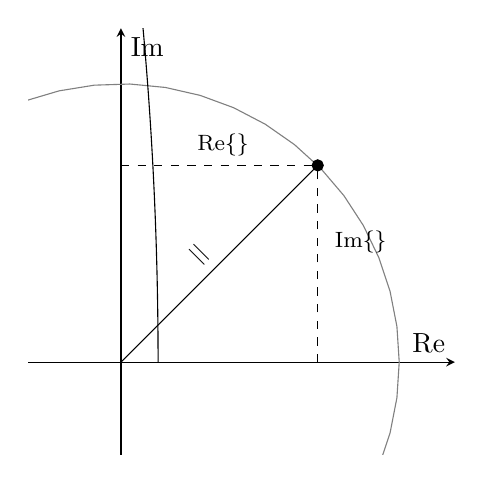
\begin{tikzpicture}
	\begin{axis}[axis equal, ymin=-0.5,xmin=-0.5,ymax=1.8,xmax=1.8,  ticks=none,
    xlabel=$\mathrm{Re}$,
    ylabel=$\mathrm{Im}$, axis lines = center, width=7cm, height=7cm]
	
    \addplot [gray,domain=0:2*pi,samples=50]({1.5*cos(deg(x))},{1.5*sin(deg(x))});
    
    \addplot [black, mark = *] coordinates {( {1.5*cos(45)}, {1.5*sin(45)} )} {};   
 %   \addplot [black, mark = *] coordinates {( {1.5*cos(-60)}, {1.5*sin(-60)} )} {};   

\addplot [black] coordinates { (0,0) ( {1.5*cos(45)}, {1.5*sin(45)} ) };
    
    \addplot [dashed,black] coordinates { ({1.5*cos(45)},0) ( {1.5*cos(45)}, {1.5*sin(45)} ) };
    
    \addplot [dashed,black] coordinates { (0,{1.5*sin(45)}) ( {1.5*cos(45)}, {1.5*sin(45)} ) };

  \draw[draw=black] (axis cs:0.2,0) arc [radius={transformdirectionx(0.2)},start angle=0,end angle=45]
  node[midway,right,inner sep=3pt,font={\footnotesize}]{$\angle \He$};

 \node at (axis cs:0.55,1.06) [above, font={\footnotesize}]{$\mathrm{Re}\{\He\}$};
 
 \node at (axis cs:1.1,0.65) [right, font={\footnotesize}]{$\mathrm{Im}\{\He\}$}; 
 
 \node at (axis cs:1.2,1.2) {$\He$};

 \node at (axis cs:0.5,0.5) [above,rotate=45,font={\footnotesize}]{$|\He|$};
\end{axis}
\end{tikzpicture}
\end{center}
\caption{The frequency response is complex-valued, and it represents a phase shift $\angle \He$ and a magnitude scaling $|\He|$ introduced by the LTI system to a complex sinusoidal signal of normalized angular frequency $\hat{\omega}$.}
\label{fig:polar_he}
\end{marginfigure}


\section{Magnitude and phase response}
The frequency response $\He \in \mathbb{C}$ is a complex-valued
function. It can be expressed in either Cartesian or polar form using Euler's formula:
\begin{equation}
\He = \mathrm{Re}\left\{\He \right\} + i\mathrm{Im}\left\{\He \right\} = \left|\He\right|e^{i \angle \He } \,\,.
\end{equation}
This is shown in Figure \ref{fig:polar_he}.


When an LTI system is applied to a complex sinusoidal signal $x[n]=A
e^{i\phi}e^{i\hat{\omega}n}$, the effect is scaling the absolute value and
shifting the phase of this signal:
\begin{align}
y[n] &= x[n]*h[n]\\
     &= \He A e^{i\phi}e^{i\hat{\omega}n} \\
     &= \underbrace{(A|\He|)}_{A'}\underbrace{e^{i(\phi + \angle \He)}}_{e^{i\phi'}} e^{i\hat{\omega} n}\\
     &= A' e^{i\phi'} e^{i\hat{\omega} n} \,\,.
\end{align}
\begin{marginfigure}
\begin{center}
\begin{tikzpicture}
	\begin{axis}[width=7cm,domain=(-3.14):(3.14),samples=200, xmin=-4,xmax=4, ymin=0,ymax=1.2,
    legend style={draw=none,at={(.99,.1)},anchor=south east},
        xlabel={$\hat{\omega}$},
	    ylabel={$|\He|$},
        axis x line=center, 
    axis y line=middle, 
    xtick={-3.14,0,3.14},
    xticklabels={$-\pi$,0,$\pi$}    
    ]
    \addplot[blue] {0.75+0.25*cos(deg(x))};
    \end{axis}
\end{tikzpicture}
\begin{tikzpicture}
	\begin{axis}[width=7cm,domain=(-3.14):(3.14),samples=200, xmin=-4,xmax=4, ymin=-3.3,ymax=3.3,
    legend style={draw=none,at={(.99,.1)},anchor=south east},
        xlabel={$\hat{\omega}$},
	    ylabel={$\angle \He$},
        axis x line=center, 
    axis y line=middle, 
    xtick={-3.14,0,3.14},
    xticklabels={$-\pi$,0,$\pi$}    
    ]
    \addplot[blue] {-x};
    \end{axis}
\end{tikzpicture}
\end{center}
\caption{An example frequency response. Top: The magnitude response of the LTI system $|\He|$. Bottom: The phase response of the system $\angle \He$.}
\label{fig:he_example_lpf}
\end{marginfigure}

The output signal is still a complex sinusoidal signal with the same
frequency, but the amplitude $A$ is scaled by a factor of $|\He|$, and the
phase is shifted by a factor $\angle \He$. The magnitude of the
frequency response $|\He|$ is called the \emph{\index{magnitude
response}{magnitude response}}:
\begin{equation}
\boxed{
|\He|=\sqrt{\Re\{\He\}^2+\Im\{\He\}^2}
} \,\,,
\end{equation}
and the phase $\angle \He$ is called
the \emph{\index{phase response}{phase response}}
\begin{equation}
\boxed{
\angle \He = \tan^{-1}\left(\frac{\Im\{\He\}}{\Re\{\He\}}\right)
} \,\,.
\end{equation}
of the LTI system. 

Figure \ref{fig:he_example_lpf} shows an example frequency response
for a low-pass filter, which reduces the absolute value of complex
sinusoidal signals with high frequencies near
$\hat{\omega}=\pm \pi$. The filter also introduces a phase shift,
which is described by a linear slope. We'll later see that a linear
slope means that the system applies a time-shift to the input signal
signal.

%\newpage
\section{Example: Low-pass filter}

Let's find the frequency response of the finite impulse response (FIR)
filter, which has an impulse response defined as:
\begin{equation}
h[n] = \left\{\begin{array}{cc}
1 & n=0\\
2 & n=1\\
1 & n=2\\
0 & \mathrm{otherwise}
\end{array} \,\,.
\right.
\end{equation}
\begin{marginfigure}
\begin{center}
        \begin{tikzpicture}
        \begin{axis}[width=6cm,height=6cm,ymin=0,ymax=2.5,xmin=-2,xmax=10,
    xlabel={$n$}, ylabel={$h[n]$}, axis lines = center]
    
   \addplot+[ycomb] plot coordinates {(-2,0) (-1,0) (0,1) (1,2) (2,1) (3,0) (4,0) (5,0)};
        \end{axis}
        \end{tikzpicture}
\end{center}
\caption{The impulse response $h[n]$ of a discrete-time low-pass filter.}
\label{fig:lp_ex}
\end{marginfigure}
\noindent Another way we can specify the impulse response is as a sum of unit impulses:
\begin{equation}
h[n] = \delta[n] + 2\delta[n-1] + \delta[n-2]
\end{equation}
The impulse response of the filter is shown in Figure \ref{fig:lp_ex}.

The frequency response can be determined using Equation \ref{eq:dt_fr}:
\begin{align}
\He &= \sum_{k=0}^{2} h[k] e^{-i\hat{\omega}k}\\
    &= h[0]e^{-i\hat{\omega}0} + h[1]e^{-i\hat{\omega}1} + h[2]e^{-i\hat{\omega}2}\\
    &= 1 + 2 e^{-i\hat{\omega}} + e^{-i2\hat{\omega}} \,\,.
\end{align}
We can tidy this up a bit by multiplying the equation with
$1=e^{-i\hat{\omega}}e^{i\hat{\omega}}$ so that we get a conjugate
symmetric pairing of complex exponential functions, which allows us to
represent $\He$ conveniently in polar form:
\begin{align}
\He &=  e^{-i\hat{\omega}}\left(e^{i\hat{\omega}} + 2 + e^{-i\hat{\omega}}\right)\\
    &= \underbrace{[2+2\cos(\hat{\omega})]}_{\mathrm{magnitude}}\underbrace{e^{-i\hat{\omega}}}_{\mathrm{phase}} \,\, _.
\end{align}
The magnitude response is $|\He|=2+2\cos(\hat{\omega})$ and the phase
response is $\angle \He = -\hat{\omega}$. These are shown in
Figure \ref{fig:lp_mr_fr}.
\begin{marginfigure}
\begin{center}
\begin{tikzpicture}
	\begin{axis}[width=7cm,domain=(-3.14):(3.14),samples=200, xmin=-4,xmax=4, ymin=0,ymax=5,
    legend style={draw=none,at={(.99,.1)},anchor=south east},
        xlabel={$\hat{\omega}$},
	    ylabel={$|\He|$},
        axis x line=center, 
    axis y line=middle, 
    xtick={-3.14,0,3.14},
    xticklabels={$-\pi$,0,$\pi$}    
    ]
    \addplot[blue] {2+2*cos(deg(x))};
    \end{axis}
\end{tikzpicture}
\begin{tikzpicture}
	\begin{axis}[width=7cm,domain=(-3.14):(3.14),samples=200, xmin=-4,xmax=4, ymin=-3.3,ymax=3.3,
    legend style={draw=none,at={(.99,.1)},anchor=south east},
        xlabel={$\hat{\omega}$},
	    ylabel={$\angle \He$},
        axis x line=center, 
    axis y line=middle, 
    xtick={-3.14,0,3.14},
    xticklabels={$-\pi$,0,$\pi$}    
    ]
    \addplot[blue] {-x};
    \end{axis}
\end{tikzpicture}
\end{center}
\caption{Magnitude and phase response of low pass filter $\{h[n]\}_{n=0}^{2} = \{1,2,1\}$.}
\label{fig:lp_mr_fr}
\end{marginfigure}

Based on the magnitude response, we can see that the filter is
a \emph{low-pass filter}. It reduces the magnitude of high frequency
spectral components of the input signal. At frequency
$\hat{\omega}=\pm\pi$, the output signal is completely attenuated, as
$|\mathcal{H}(\pm \pi)|=0$.

The phase response has a linear slope $\angle \He =
-\hat{\omega}$. This implies that the output signal is delayed
relative to the input by a constant value. Recall that a delay to a
complex sinusoidal signal $x[n]=A e^{i\phi} e^{i\hat{\omega}n} $ is:
\begin{equation}
x[n-n_0] = A e^{i\phi} e^{i\hat{\omega} (n-n_0)} = e^{-i\hat{\omega}n_0}x[n] \,\,.
\end{equation}
This means that a delay by one sample $n_0=1$ will correspond to the phase
response of $\angle \He = -\hat{\omega}$.


\section{Example: High-pass filter}
\begin{marginfigure}
\begin{center}
        \begin{tikzpicture}
        \begin{axis}[width=6cm,height=6cm,ymin=-1.5,ymax=1.5,xmin=-2,xmax=10,
    xlabel={$n$}, ylabel={$h[n]$}, axis lines = center]
    
   \addplot+[ycomb] plot coordinates {(-2,0) (-1,0) (0,1) (1,-1) (2,0) (3,0) (4,0) (5,0)};
        \end{axis}
        \end{tikzpicture}
\end{center}
\caption{The impulse response of a high-pass filter $h[n]=\delta[n]-\delta[n-1]$.}
\label{fig:first_diff}
\end{marginfigure}

A first difference system is defined as follows:
\begin{align}
y[n] & = x[n] - x[n-1] \,\,.
\end{align}
This is equivalent to a FIR filter with an impulse response $h[n]=\delta[n]-\delta[n-1]$. This is shown in Figure \ref{fig:first_diff}.

Using Equation \ref{eq:dt_fr}, we obtain the frequency response:
\begin{align}
\He & = \sum_k h[k] e^{-i\hat{\omega}k}\\
    & = 1 -  e^{-i\hat{\omega}} \,\,.
\end{align}
If we multiply this with $1=e^{-i\frac{\hat{\omega}}{2}}e^{i\frac{\hat{\omega}}{2}}$, we obtain:
\begin{equation}
\He = e^{-i\frac{\hat{\omega}}{2}}\left(e^{i\frac{\hat{\omega}}{2}}-e^{-i\frac{\hat{\omega}}{2}}\right) \,\,.
\end{equation}
We know that $\frac{1}{2i}(e^{i\alpha} - e^{-i\alpha}) = \sin(\alpha)$, therefore:
\begin{equation}
\He = e^{-i\frac{\hat{\omega}}{2}} 2i \sin(\frac{\hat{\omega}}{2}) \,\,.
\end{equation}
We also know that $i=e^{i\frac{\pi}{2}}$, so 
\begin{equation}
\He = 2\sin(\frac{\hat{\omega}}{2}) e^{-i\frac{1}{2}(\hat{\omega}-\pi)} \,\,.
\end{equation}
In order to inspect the magnitude and phase response, we need to
obtain the frequency response in the following form:
\begin{equation}
\He =|\He |e^{i\angle \He} \,\,.
\end{equation} 

\begin{marginfigure}
\begin{center}
\begin{tikzpicture}
	\begin{axis}[width=7cm,domain=(-3.14):(3.14),samples=200, xmin=-4,xmax=4, ymin=0,ymax=2.5,
    legend style={draw=none,at={(.99,.1)},anchor=south east},
        xlabel={$\hat{\omega}$},
	    ylabel={$|\He|$},
        axis x line=center, 
    axis y line=middle, 
    xtick={-3.14,0,3.14},
    xticklabels={$-\pi$,0,$\pi$}    
    ]
    \addplot[blue] {2*abs(sin(deg(x/2)))};
    \end{axis}
\end{tikzpicture}

\begin{tikzpicture}
	\begin{axis}[width=7cm,domain=(-3.14):(3.14),samples=200, xmin=-4,xmax=4, ymin=-2,ymax=2,
    legend style={draw=none,at={(.99,.1)},anchor=south east},
        xlabel={$\hat{\omega}$},
	    ylabel={$\angle \He$},
        axis x line=center, 
    axis y line=middle, 
    xtick={-3.14,0,3.14},
    xticklabels={$-\pi$,0,$\pi$},    
    ytick={-1.507,1.507},
    yticklabels={$-\frac{\pi}{2}$,$\frac{\pi}{2}$}
]
    \addplot[blue] {rad(atan(sin(deg(x))/(1-cos(deg(x)))))};

\end{axis}
\end{tikzpicture}
\end{center}
\caption{Top: The magnitude response of the high-pass filter. Bottom: The phase response of the same filter.}
\label{fig:hp_filter_ex}
\end{marginfigure}

\noindent We can do this using a phase shift by $\pi$ to flip the phase $-1 = e^{-i\pi}$. This allows us to take into account the fact that $\sin(\hat{\omega}/2)$ is negative when $-\pi < \hat{\omega} < 0$. The frequency response can now be written as:
\begin{equation}
\He = \left\{ 
  \begin{array}{llr}
    2\left|\sin\left(\frac{\hat{\omega}}{2}\right)\right|
    e^{-i\frac{1}{2}(\hat{\omega}-\pi)} & \mathrm{when} & 0
    < \hat{\omega} < \pi \\
    2\left|\sin\left(\frac{\hat{\omega}}{2}\right)\right|
    e^{-i\frac{1}{2}(\hat{\omega}+\pi)} & \mathrm{when} & -\pi
    < \hat{\omega} \le 0 \end{array} \,\, _.
\right.
\end{equation}
The magnitude response is thus:
\begin{equation}
|\He|=2\left|\sin\left(\frac{\hat{\omega}}{2}\right)\right| \,\, _,
\end{equation} 
and the phase response is:
\begin{equation}
\angle \He = \left\{ 
  \begin{array}{lcr}
    -\frac{1}{2}\hat{\omega} + \frac{\pi}{2}  & \mathrm{when} & 0 < \hat{\omega} < \pi \\
    -\frac{1}{2}\hat{\omega} - \frac{\pi}{2}  & \mathrm{when} & -\pi < \hat{\omega} \le 0 \\
  \end{array} \,\, _.
\right.
\end{equation}
The magnitude and phase response is shown in
Figure \ref{fig:hp_filter_ex}. It completely removes the zero-frequency
component of the signal, and reduces the amplitudes of low frequency
spectral components. High frequency spectral components of the input
signal will be amplified. For input signal spectral components with
frequencies at $\hat{\omega}=\pm \pi$, the filter output signal
spectral components will have twice the original magnitude.

This type of filter is called a \emph{\index{high-pass
filter}{high-pass filter}}, as it attenuates low frequency spectral
components relative to high frequency spectral components.

\section{Example: band-pass filter}

Let's now investigate the frequency response of the following filter:
\begin{align}
y[n] & = 0.5 x[n+1] - 0.5 x[n-1] \,\,.
\end{align}
The impulse response  $h[n]=0.5\delta[n+1]-0.5\delta[n-1]$ of this system is shown in Figure \ref{fig:example0_bpf_h}.
\begin{marginfigure}
\begin{center}
        \begin{tikzpicture}
        \begin{axis}[width=6cm,height=6cm,ymin=-1.5,ymax=1.5,xmin=-4,xmax=4,
    xlabel={$n$}, ylabel={$h[n]$}, axis lines = center]
    
   \addplot+[ycomb] plot coordinates {(-3,0) (-2,0) (-1,0.5) (0,0) (1,-0.5) (2,0) (3,0) (3,0)};
        \end{axis}
        \end{tikzpicture}
\end{center}
\caption{The impulse response of a simple band-pass filter.}
\label{fig:example0_bpf_h}
\end{marginfigure}

\begin{marginfigure}
\begin{center}
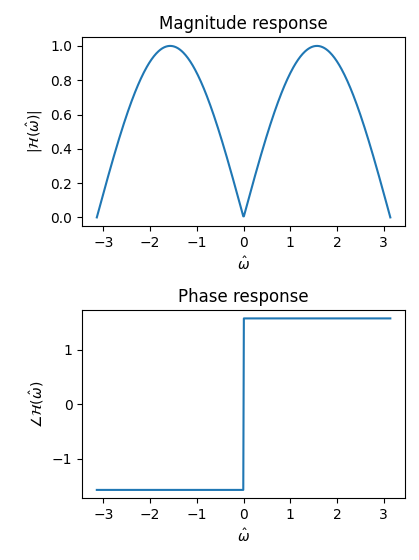
\includegraphics[width=\textwidth]{code/019_frequency_response/bpf_fresp.png}
\end{center}
\caption{The frequency response of the band-pass filter $h[n]=0.5\delta[n+1]-0.5\delta[n-1]$. Top: the magnitude response. Bottom: The phase response.}
\label{fig:example_bpf_fresp}
\end{marginfigure}

Using Equation \ref{eq:dt_fr}, we obtain the frequency response:
\begin{align}
\He & = \sum_k h[k] e^{-i\hat{\omega}k}\\
    & = 0.5e^{i\hat{\omega}} -  0.5e^{-i\hat{\omega}} \\
    &= i \sin(\hat{\omega}) \,\,.
\end{align}
If we wanted to investigate this analytically, we could use the type
of analysis that did in the previous example. We'll write a little
Python script instead to plot the magnitude and phase response. This is shown in Listing \ref{lst:freq_resp_ex}.

The plot produced is shown in Figure \ref{fig:example_bpf_fresp}. From
the magnitude response plot, we can see that this filter reduces the
magnitudes of high and low frequency spectral components of the input
signal near $\hat{\omega}=0$ and $\hat{\omega}=\pm \pi$. However, the
spectral components with frequencies near
$\hat{\omega}=\pm \frac{\pi}{2}$ are unchanged in magnitude. The phase
response is flat, except for a discontinuity at 0, where
the phase switches from $-\frac{\pi}{2}$ to $\frac{\pi}{2}$ to account
for the sign of the $\sin$ function.

This type of filter that only lets through spectral components of
the signal within a range of frequencies is called a \emph{\index{band-pass
filter}{band-pass
filter}}. 

\lstinputlisting[language=Python,caption={\texttt{019\_frequency\_response/example\_bpf.py}},label=lst:freq_resp_ex]{code/019_frequency_response/example_bpf.py}

\section{Example: Delay filter}

A delay system is defined as:
\begin{marginfigure}
\begin{center}
        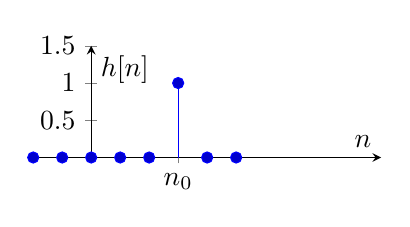
\begin{tikzpicture}
        \begin{axis}[width=6cm,height=3cm,ymin=0,ymax=1.5,xmin=-2,xmax=10,
        xtick={3},
        xticklabels={$n_0$},
    xlabel={$n$}, ylabel={$h[n]$}, axis lines = center]
    
   \addplot+[ycomb] plot coordinates {(-2,0) (-1,0) (0,0) (1,0) (2,0) (3,1) (4,0) (5,0)};
        \end{axis}
        \end{tikzpicture}
\end{center}
\caption{The impulse response of a time-shift system.}
\label{fig:shift_imp_resp}
\end{marginfigure}
\begin{marginfigure}
\begin{center}
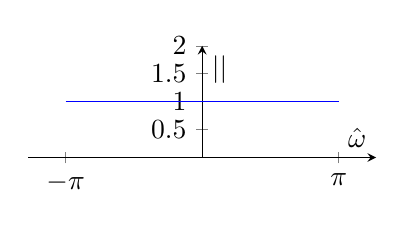
\begin{tikzpicture}
	\begin{axis}[width=6cm,height=3cm,domain=(-3.14):(3.14),samples=200, xmin=-4,xmax=4, ymin=0,ymax=2,
    legend style={draw=none,at={(.99,.1)},anchor=south east},
        xlabel={$\hat{\omega}$},
	    ylabel={$|\He|$},
        axis x line=center, 
    axis y line=middle, 
    xtick={-3.14,0,3.14},
    xticklabels={$-\pi$,0,$\pi$}    
    ]
    \addplot[blue] {1};
    \end{axis}
\end{tikzpicture}
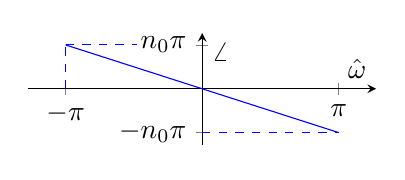
\begin{tikzpicture}
	\begin{axis}[width=6cm, height=3cm,domain=(-3.14):(3.14),samples=200, xmin=-4,xmax=4, ymin=-8,ymax=8,
    legend style={draw=none,at={(.99,.1)},anchor=south east},
        xlabel={$\hat{\omega}$},
	    ylabel={$\angle \He$},
        axis x line=center, 
    axis y line=middle, 
    xtick={-3.14,0,3.14},
    xticklabels={$-\pi$,0,$\pi$},    
    ytick={-6.28,6.28},
    yticklabels={$-n_0\pi$,$n_0\pi$}
]
    \addplot[blue] {-2*x};
    \addplot [dashed,blue] coordinates { (-3.14,0) ( -3.14, 6.28 ) };
    \addplot [dashed,blue] coordinates { (-3.14,6.28) ( -1.5, 6.28 ) };
\addplot [dashed,blue] coordinates { (0,{-2*3.14}) ( 3.14, {-2*3.14} ) };
\end{axis}
\end{tikzpicture}
\end{center}
\caption{The frequency response of a time-delay filter.}
\label{fig:shift_freq_resp}
\end{marginfigure}

\begin{equation}
y[n] = x[n-n_0] \,\,.
\end{equation}
This has a unit impulse $h[n]=\delta[n-n_0]$ (shown in
Figure \ref{fig:shift_imp_resp}). Using Equation \ref{eq:dt_fr}, we
obtain the following frequency response:
\begin{align}
\He & = \sum_k h[k] e^{-i\hat{\omega}k}\\
    & = \sum_k \delta[k-n_0] e^{-i\hat{\omega}k}\\
    & = e^{-i\hat{\omega}n_0} \,\,.
\end{align}

The magnitude response is $|\He|=1$ and the phase response is
$\angle \He = -\hat{\omega}n_0$. This is shown in
Figure \ref{fig:shift_freq_resp}. This filter does not modify the
magnitude of any spectral components. However, it applies a phase
shift to spectral components, which results in a time delay.

\begin{marginfigure}
\begin{center}

\begin{tikzpicture}
	\begin{axis}[domain=(-1):(1),samples=300,
        width=6cm,
        height=4cm,
    ymin=0,ymax=1.5,
        xlabel={$t$},
        ylabel={$h(t)$},
        axis x line=center, 
        axis y line=center,
        ytick={0,1},
        yticklabels={0,$\frac{1}{T}$}, 
        xtick={-0.5,0.5},
        xticklabels={$-\frac{T}{2}$,$\frac{T}{2}$}
    ]

    \addplot[blue] {(x>-0.5)*(x<0.5)};
\end{axis}
\end{tikzpicture}

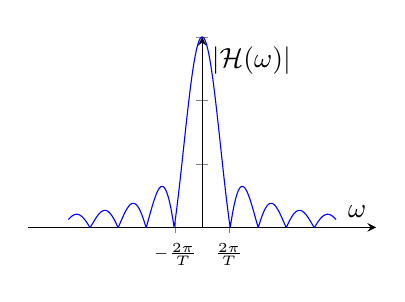
\begin{tikzpicture}

\begin{axis}[
        domain=(-10):(10),
        samples=300,
        width=6cm,
        xmin=-13,
        xmax=13,
        height=4cm,        
        xlabel={$\omega$},
        ylabel={$|\mathcal{H}(\omega)|$},
        axis x line=center, 
        axis y line=center, 
        yticklabels={,,,},
        tick label style={font=\tiny},
        xtick={-2.0,2.0},
        xticklabels={$-\frac{2\pi}{T}$,$\frac{2\pi}{T}$}
    ]
    \addplot[blue] {abs(2*sin(0.5*3*deg(x))/x)};
\end{axis}
\end{tikzpicture}
\\
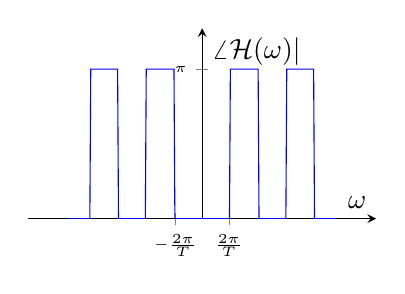
\begin{tikzpicture}
	\begin{axis}[
        domain=(-10):(10),
        samples=300,
        width=6cm,
        xmin=-13,
        xmax=13,
        height=4cm,        
        xlabel={$\omega$},
        ylabel={$\angle \mathcal{H}(\omega)|$},
        axis x line=center, 
        axis y line=center,
        ytick={0,3.14},
        tick label style={font=\tiny},  
        yticklabels={0,$\pi$},
        xtick={-2.0,2.0},
        xticklabels={$-\frac{2\pi}{T}$,$\frac{2\pi}{T}$},
        ymax=4,
        ymin=0
    ]
    \addplot[blue] {(-1*sign(sin(0.5*3*deg(x))/x)+1.0)*3.14/2.0};
\end{axis}
\end{tikzpicture}

\end{center}
\caption{Top: the impulse response of an averaging filter. Middle: The magnitude response. Bottom: The phase response.}
\label{fig:sinc_lp}
\end{marginfigure}

This may seem trivial now, but the frequency domain representation for
a time-shift will later be useful; when defining more advanced,
fractional sample, time-shift filters for discrete-time signals. In
this case, $n_0 \in \mathbb{R}$ is not an integer. We'll need to
define the inverse discrete-time Fourier transform in order to derive
the filter impulse response in this case.


\section{Example: Continuous-time low-pass filter}

Consider a continuous-time LTI system, which uniformly averages the
input signal around a region of length $T$:
\begin{equation}
y(t) = \frac{1}{T}\int_{-\frac{T}{2}}^{\frac{T}{2}} x(t-\tau)d\tau \,\,.
\end{equation}
This has the following an impulse response:
\begin{equation}
h(t)=\frac{1}{T}[u(t+T/2)-u(t-T/2)] \,\,.
\label{eq:rect_fun}
\end{equation}
This is the familiar rectangular function. Using
Equation \ref{eq:fresp_ct}, we obtain the following frequency
response\footnote{See the Fourier transform chapter for derivation of Equation \ref{eq:rect_fun_ft}.}:
\begin{equation}
\mathcal{H}(\omega)=\frac{2\sin(\omega T/2)}{\omega T} \,\, _.
\label{eq:rect_fun_ft}
\end{equation}
Note that this is a continuous-time frequency response. Our frequency
variable is angular frequency (radians per second). The frequency
response is a sinc-function, as shown in
Figure \ref{fig:sinc_lp}. This is a low-pass filter, as this filter
reduces the magnitude of spectral components of the input signal
$x(t)$ with higher frequencies.


\section{Example: Time symmetric running average filter}

Let's now look at a discrete-time version of the previous
continuous-time filter, the time symmetric running average
system. This system averages $M=2N+1$ values of the input signal
$x[n]$:
\begin{equation}
y[n] = \frac{1}{M} \sum_{k=-N}^{N} x[n-k] \,\, _.
\end{equation}

\begin{marginfigure}
\begin{center}
        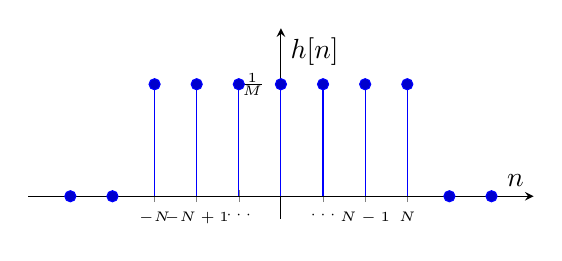
\begin{tikzpicture}
        \begin{axis}[width=8cm,height=4cm,ymin=-0.2,ymax=1.5,xmin=-6,xmax=6,
        ytick={0,1}, yticklabels={0,$\frac{1}{M}$},
        xtick={-3,-2,-1,0,1,2,3},
        xticklabels={$-N$,$-N+1$,$\cdots$,$0$,$\cdots$,$N-1$,$N$},
        tick label style={font=\tiny},
        xlabel={$n$}, ylabel={$h[n]$}, axis lines = center]
        \addplot+[ycomb] plot coordinates {(-5,0) (-4,0) (-3,1) (-2,1) (-1,1) (0,1) (1,1)  (2,1) (3,1) (4,0) (5,0)};
        \end{axis}
        \end{tikzpicture}
\end{center}
\caption{The impulse response of a discrete-time running average filter.}
\label{fig:rmf_ir}
\end{marginfigure}

We can easily see that this is an LTI system with an impulse response:
\begin{equation}
h[n] = \frac{1}{M}\sum_{k=-N}^{N}\delta[n-k] \,\, _.
\end{equation}
The impulse response $h[n]$ of the system is shown in
Figure \ref{fig:rmf_ir}. This type of filter is often used to smooth
noisy signals. It will also later on play an important role in
determining the frequency response of a discrete Fourier transform.

Using Equation \ref{eq:dt_fr}, we can find the frequency response of this filter:
\begin{equation}
\He = \sum_{k=-N}^N \frac{1}{M} e^{-i\hat{\omega}k} \,\, _.
\end{equation}
Let's set $c=1/M$, $\alpha=e^{i\hat{\omega}}$, and $S=\He$. By doing
some algebraic manipulations, we can find a closed form solution:
\begin{align}
S &= c \alpha^{-N} + c \alpha^{-N+1} + \cdots+ c +\cdots + c \alpha^{N-1} + c\alpha^N \\
\alpha S &= c \alpha^{-N+1} + c \alpha^{-N+2} + \cdots+ c +\cdots + c \alpha^{N} + c\alpha^{N+1} \\
S-\alpha S &= c\alpha^{-N} - c\alpha^{N+1}\\
S(1-\alpha) &= c(\alpha^{-N}-\alpha^{N+1})\\
S &= c \frac{\alpha^{-N} - \alpha^{N+1}}{1-\alpha} \,\, _.
\label{eq:gs_sol_form}
\end{align}
This is known as the closed form solution to a \emph{\index{geometric
series}{geometric series}}. When substituting back the values of $c$,
$\alpha$, and $S$ we obtain:
\begin{equation}
\He = \frac{1}{M} \frac{e^{-i\hat{\omega}N}-e^{i \hat{\omega}(N+1)}}{1-e^{i\hat{\omega}}} \,\, _.
\end{equation}

We can once again use the trick of multiplying the complex
exponentials with $1=e^{i\hat{\omega}/2}e^{-i\hat{\omega}/2}$ on the
numerator and denominator. This allows us to create conjugate pairings
of complex exponentials:
\begin{align}
\He &= \frac{1}{M} \frac{e^{-i\hat{\omega}N}-e^{i \hat{\omega}(N+1)}}{1-e^{i\hat{\omega}}}\\
         &= \frac{1}{M} \frac{(e^{-i\hat{\omega}N}-e^{i \hat{\omega}(N+1)})[e^{i\hat{\omega}/2}e^{-i\hat{\omega}/2}] }{(1-e^{i\hat{\omega}})[e^{i\hat{\omega}/2}e^{-i\hat{\omega}/2}] }\\
         &= \frac{1}{M} \frac{\cancel{e^{i\hat{\omega}/2}}}{\cancel{e^{i\hat{\omega}/2}}} \frac{  (e^{-i\hat{\omega}(N+1/2)}-e^{i \hat{\omega}(N+1/2)}) }{(e^{-i\hat{\omega}/2} -e^{i\hat{\omega}/2} ) } \\
          &= \frac{1}{M} \frac{ e^{-i\hat{\omega}(N+1/2)}-e^{i \hat{\omega}(N+1/2)} }{e^{-i\hat{\omega}/2} -e^{i\hat{\omega}/2}  } \,\, _,
\end{align}
\begin{marginfigure}
\begin{center}
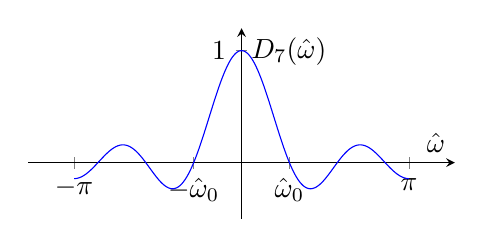
\begin{tikzpicture}
	\begin{axis}[width=7cm,
        height=4cm,
        domain=(-3.14):(3.14),
        samples=200,
        xmin=-4,
        xmax=4,
        ymin=-0.5,
        ymax=1.2,
    legend style={draw=none,at={(.99,.1)},anchor=south east},
        xlabel={$\hat{\omega}$},
	    ylabel={$D_{7}(\hat{\omega})$},
        axis x line=center, 
    axis y line=middle,
        ytick={0,1},
    xtick={-3.14,-0.897,0,0.897,3.14},
    xticklabels={$-\pi$,$-\hat{\omega}_0$,0,$\hat{\omega}_0$,$\pi$}    
    ]
    \addplot[blue] {sin(deg(x*(3+0.50000001)))/(7*sin(1e-6+deg(x/2.0)))};
    \end{axis}
\end{tikzpicture}

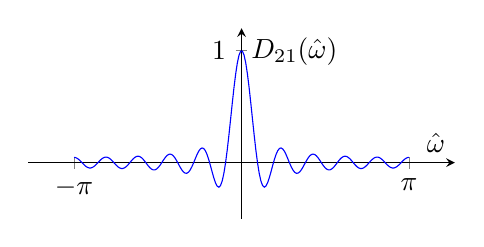
\begin{tikzpicture}
	\begin{axis}[width=7cm,
        height=4cm,
        domain=(-3.14):(3.14),
        samples=200,
        xmin=-4,
        xmax=4,
        ymin=-0.5,
        ymax=1.2,
    legend style={draw=none,at={(.99,.1)},anchor=south east},
        xlabel={$\hat{\omega}$},
	    ylabel={$D_{21}(\hat{\omega})$},
        axis x line=center, 
    axis y line=middle,
        ytick={0,1},
    xtick={-3.14,0,3.14},
    xticklabels={$-\pi$,0,$\pi$}    
    ]
    \addplot[blue] {sin(deg(x*(10+0.50000001)))/(21*sin(1e-6+deg(x/2.0)))};
    \end{axis}
\end{tikzpicture}

\end{center}
\caption{The Dirichlet kernel $D_{7}(\hat{\omega})$ and $D_{21}(\hat{\omega})$. The first zero-crossings $\pm\hat{\omega}_0$ are 
depicted for $D_{7}(\hat{\omega})$, which indicate the bandwidth of the filter.}
\label{fig:dir_kernel}
\end{marginfigure}

\noindent which then allows us to use $\sin(\theta)=\frac{1}{2i}(e^{i\theta}-e^{-i\theta})$ 
to relate the symmetric pairs to $\sin$ functions:
\begin{align}
\He &= \frac{1}{M} \frac{\cancel{-2i}}{\cancel{-2i}} \frac{ \sin(\hat{\omega} (N+1/2)) }{\sin(\hat{\omega}/2)} = D_{M}(\hat{\omega}) \,\,.
\end{align}
The function $D_M(\hat{\omega})$ is defined as (recall that $M=2N+1$):
\begin{equation}
\boxed{
D_M(\hat{\omega}) = \frac{1}{M}\frac{ \sin(\hat{\omega}M/2) }{\sin(\hat{\omega}/2)}
}\label{eq:dirikereq} \,\, _.
\end{equation}
It is sometimes referred to as the \emph{\index{periodic
sinc}{periodic sinc}} function, and sometimes as
the \emph{\index{Dirichlet kernel}{Dirichlet kernel}}\footnote{Note that there
are several conflicting definitions of the Dirichlet kernel. I am
using the one consistent with the Scipy
implementation \texttt{scipy.special.diric(x,n)}.}.

Equation \ref{eq:dirikereq} may at first appear problematic at
$\hat{\omega}=0$, which results in $D_M(0)=0/0$. 
This can be resolved using L'H\^opital's rule:
\begin{equation}
\lim_{x\rightarrow c} \frac{f(x)}{g(x)} = \lim_{x\rightarrow c} \frac{f'(x)}{g'(x)} \,\, _.
\end{equation}
From this it follows that:
\begin{equation}
D_M(0) = 1 \,\,.
\end{equation}
Figure \ref{fig:dir_kernel} shows a plot of the Dirichlet kernel for
$M=7$ and $M=21$, which shows that the width of the main lobe becomes
more narrow as $M$ is increased. The location of the first
zero-crossing of $D_M(\hat{\omega}_0)=0$ is at
$\hat{\omega}_0=2\pi/M$. This is a demonstration
of \emph{\index{time-frequency ambiguity}{time-frequency ambiguity}},
i.e., the inverse relationship between the width of a signal in time
domain and frequency domain.

\begin{marginfigure}
\begin{center}
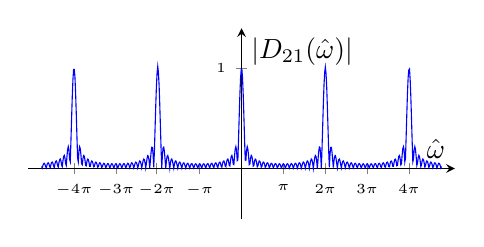
\begin{tikzpicture}
	\begin{axis}[width=7cm,
        height=4cm,
        domain=(-15):(15),
        samples=600,
        xmin=-16,
        xmax=16,
        ymin=-0.5,
        ymax=1.4,
    legend style={draw=none,at={(.99,.1)},anchor=south east},
        xlabel={$\hat{\omega}$},
	    ylabel={$|D_{21}(\hat{\omega})|$},
        axis x line=center, 
    axis y line=middle,
        ytick={0,1},
                tick label style={font=\tiny},
    xtick={-12.56,-9.42,-6.38,-3.14,0,3.14,6.28,9.42,12.56},
    xticklabels={$-4\pi$,$-3\pi$,$-2\pi$,$-\pi$,0,$\pi$,$2\pi$,$3\pi$,$4\pi$}    
    ]
    \addplot[blue] {abs(sin(deg(x*(10+0.50000001)))/(21*sin(1e-6+deg(x/2.0))))};
    \end{axis}
\end{tikzpicture}
\end{center}
\caption{The Dirichlet kernel is $2\pi$-periodic, which is a general property of discrete-time frequency responses.}
\label{fig:dir_kernel2}
\end{marginfigure}

It can be shown that the Dirichlet kernel also arises from the Fourier
series representation of a Dirac comb signal with period $2\pi$:
\begin{equation}
D'(\hat{\omega}) = \sum_{k=-\infty}^{\infty} \delta(\hat{\omega}-2\pi k) \,\,,
\label{eq:dirac_comb_dirichlet}
\end{equation}
which has the following Fourier series representation using $M=2N+1$ terms:
\begin{equation}
D'_M(\hat{\omega}) = \frac{1}{2\pi}\sum_{k=-N}^{N} e^{i \hat{\omega} k} = \frac{1}{2\pi}\frac{ \sin(\hat{\omega}M/2) }{\sin(\hat{\omega}/2)} \,\,.
\label{eq:dirichlet2}
\end{equation}
Note that $D'_M(\hat{\omega})$ and $D_M(\hat{\omega})$ are up to a
constant the same. The proof of Equation \ref{eq:dirichlet2} is
essentially the same as the derivation of the running mean filter
frequency response shown above\footnote{The Fourier series
representation for a Dirac comb signal was discussed in the Fourier
series chapter.}. As $N\rightarrow \infty$, the location of the first
zero crossing approaches $\hat{\omega}=0$. This means that the
bandwidth of the filter approaches zero and passes through only
signals with frequencies $\hat{\omega}=2\pi k$.

From Equation \ref{eq:dirac_comb_dirichlet} it is easy to see that the Dirichlet kernel is $2\pi$-periodic. This is a general property that
applies to the frequency response of any discrete-time LTI system,
and is due to dicretization of the signal.

There is a short Python program in Listing \ref{lst:dirichlet}, which
can be used to plot the magnitude and phase response of the running
average filter. The output of this program is shown in
Figure \ref{fig:output_dirichlet}.

\begin{marginfigure}
\begin{center}
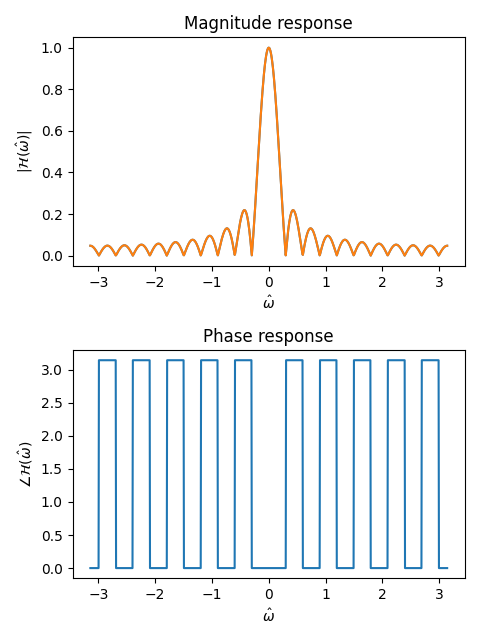
\includegraphics[width=\textwidth]{code/019_frequency_response/dirichlet21.png}
\end{center}
\caption{The output of the program in Listing \ref{lst:dirichlet}, which shows the magnitude and phase response of the 21-point running average filter. As one can see of the plot, the two methods have equivalent magnitude response.}
\label{fig:output_dirichlet}
\end{marginfigure}

\lstinputlisting[language=Python,caption={\texttt{019\_frequency\_response/dirichlet.py}},label=lst:dirichlet]{code/019_frequency_response/dirichlet.py}